\documentclass[aspectratio=169]{beamer} 
\usepackage{amsmath,amsthm}
\usepackage{graphicx,microtype,parskip}
\usepackage{caption,subcaption,multirow}
\usepackage{attrib}
\usepackage{array}

\frenchspacing

\usetheme{default}
\usecolortheme{whale}

\setbeamertemplate{navigation symbols}{}

\setbeamercolor{title}{fg=blue,bg=white}

\setbeamercolor{block title}{fg=white,bg=gray}
\setbeamercolor{block body}{fg=black,bg=lightgray}

\setbeamercolor{block title alerted}{fg=white,bg=darkgray}
\setbeamercolor{block body alerted}{fg=black,bg=lightgray}


\title{How predictable is extinction?} 
\subtitle{Forecasting species survival at million-year timescales}
\author{Peter D Smits, Seth Finnegan}
\institute{Department of Integrative Biology, University of California -- Berkeley}
\date{}


\begin{document}


\begin{frame}
  \maketitle
\end{frame}


\begin{frame}
  \frametitle{Foundational assertion of conservation paleobiology }

  \begin{center}
    \begin{LARGE}
      By studying the \alert{past}, \\we can better predict the \alert{future}.
    \end{LARGE}
  \end{center}

\end{frame}


\begin{frame}
  \frametitle{What are we predicting?}

  \begin{center}
    \begin{LARGE}
      Extinction is \alert{hard} to predict, but is \alert{important} to conservation decisions.
    \end{LARGE}
  \end{center}

\end{frame}


\begin{frame}
  \frametitle{Predicting extinction}

  \begin{itemize}[<+->]
    \item A taxon with a \alert{greater than average} global geographic range is likely to \alert{survive for longer} than a taxon with \alert{less than average} global geographic range.
    \item A taxon's global geographic range can change over time.
    \item What happens to extinction risk as a taxon changes geographic range? How is extinction risk impacted if that taxon's global geographic range has recently \alert{increased} or \alert{decreased}?
  \end{itemize}

\end{frame}


\begin{frame}
  \frametitle{Data being analyzed: Neptune database}

  \begin{columns}
    \begin{column}{0.1\textwidth}
      \begin{center}
        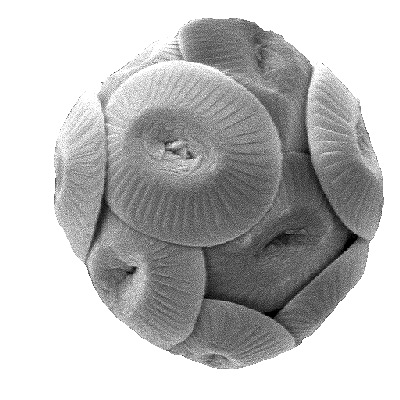
\includegraphics[width=\textwidth,height=0.15\textheight,keepaspectratio=true]{figure/calc}

        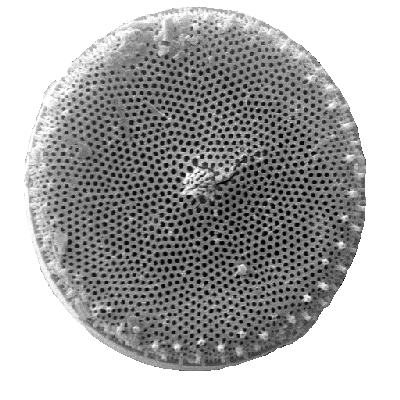
\includegraphics[width=\textwidth,height=0.15\textheight,keepaspectratio=true]{figure/diatom}

        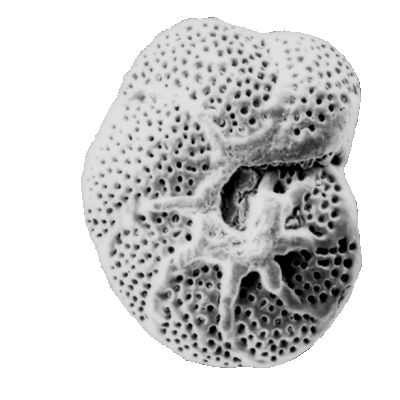
\includegraphics[width=\textwidth,height=0.15\textheight,keepaspectratio=true]{figure/foram}

        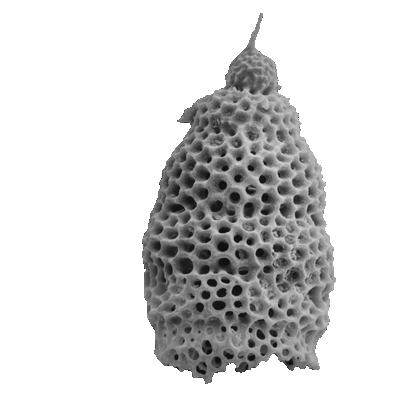
\includegraphics[width=\textwidth,height=0.15\textheight,keepaspectratio=true]{figure/rad}

        \attrib{\footnotesize{UCL}}
      \end{center}
    \end{column}
    \begin{column}{0.4\textwidth}
      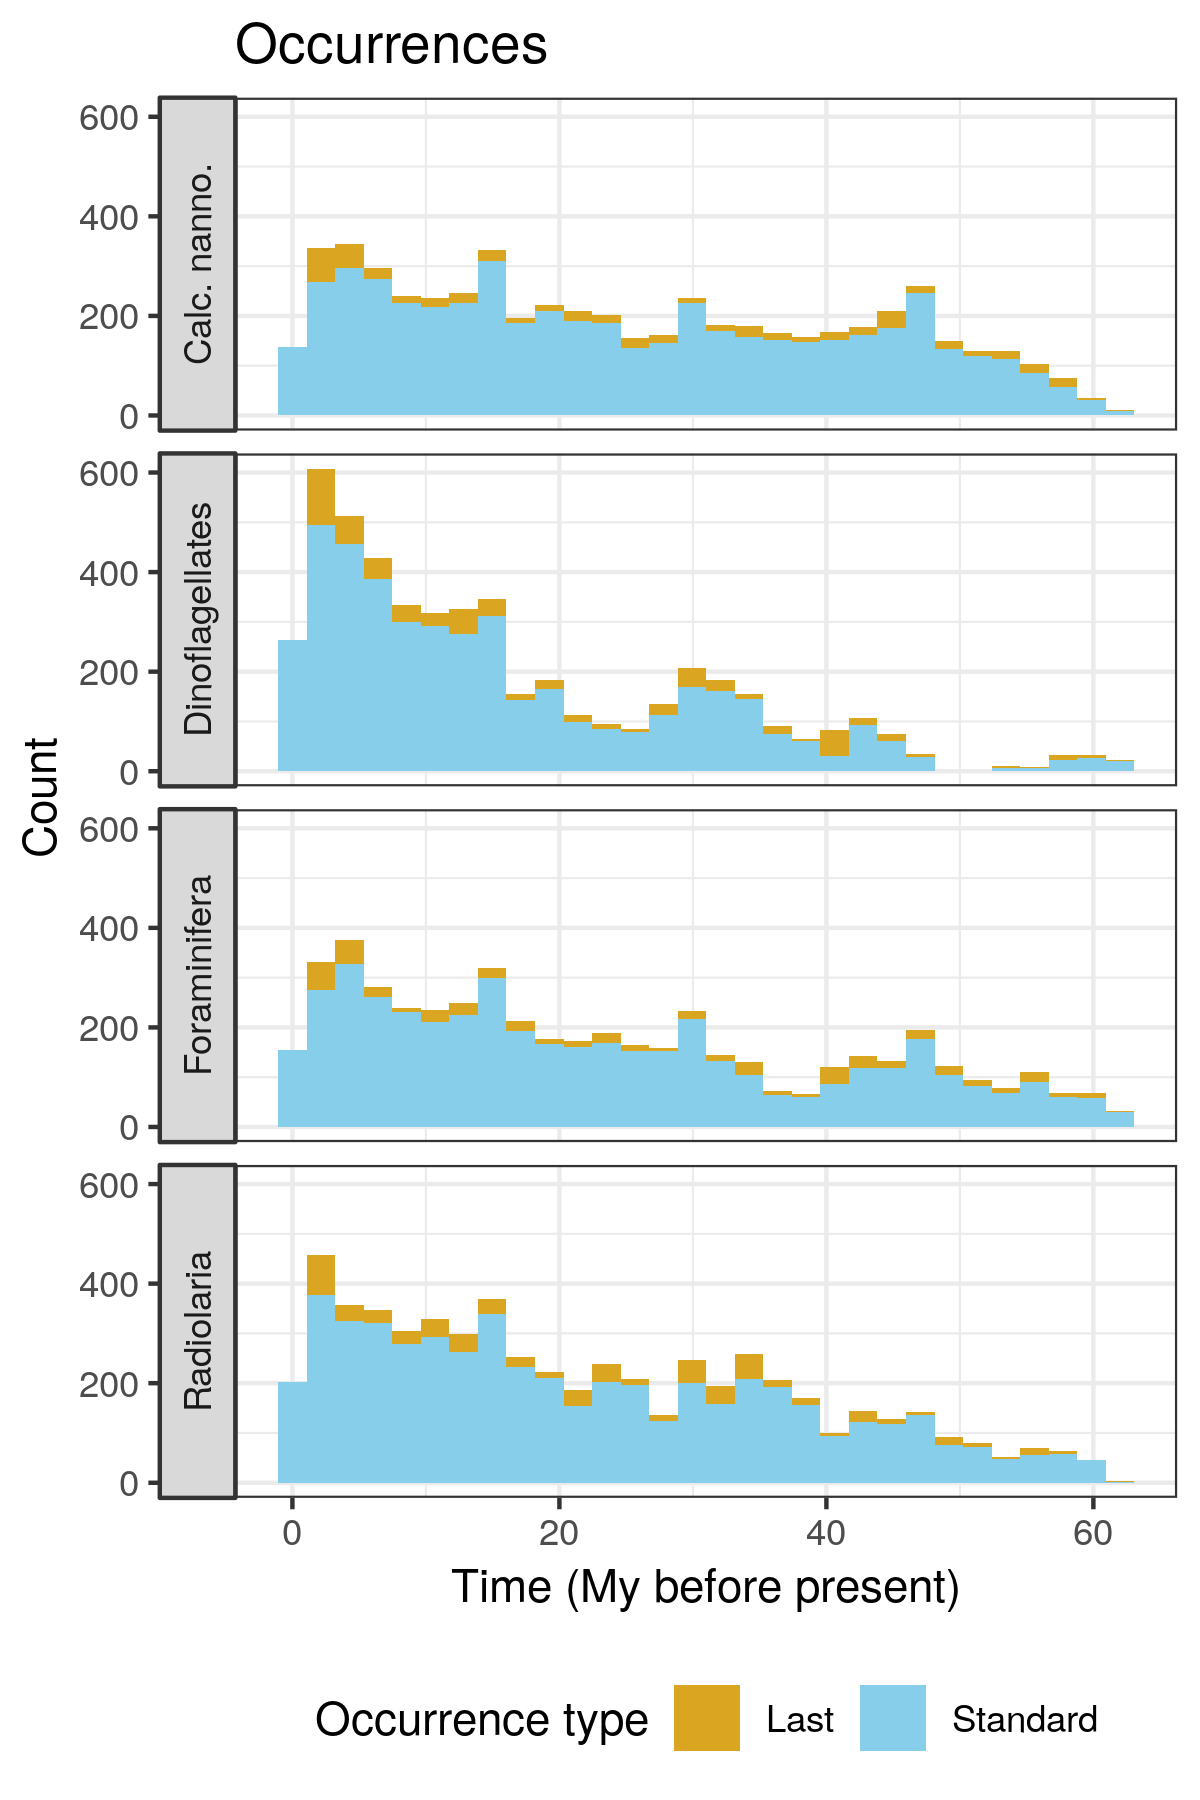
\includegraphics[width=\textwidth,height=0.7\textheight,keepaspectratio=true]{../results/figure/occ_time_label_full}
    \end{column}
    \begin{column}{0.4\textwidth}
      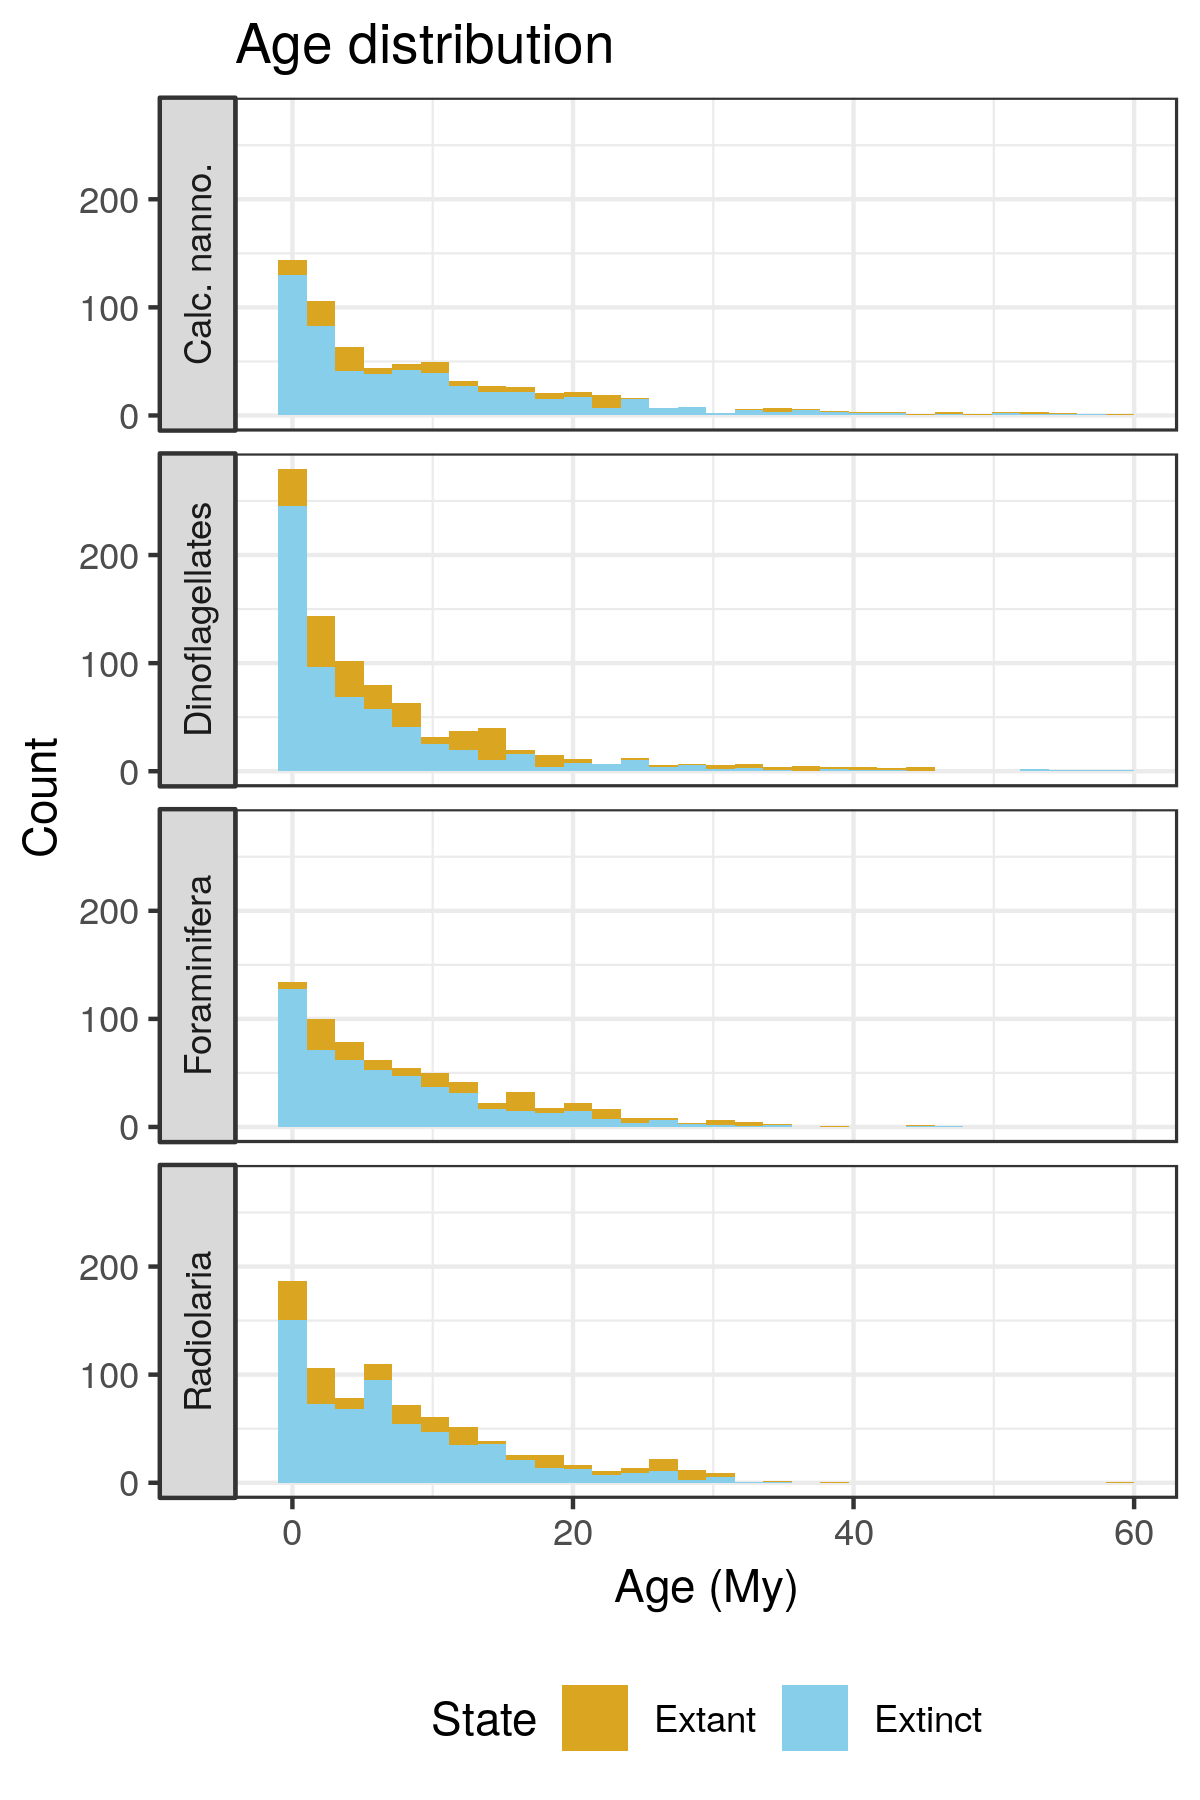
\includegraphics[width=\textwidth,height=0.7\textheight,keepaspectratio=true]{../results/figure/age_label_full}
    \end{column}
  \end{columns}

  \footnotesize{Global occurrences from Deep Sea Drilling Program and Ocean Drilling Project. -- Lazarus. 1994. Math. Geo.; Spencer-Cervato. 1999. Palaeo. Elec.}

\end{frame}


\begin{frame}
  \frametitle{How we're analyzing the data}

  \begin{itemize}%[<+->]
    \item Encoding the past
      \begin{itemize}
        \item Change in geographic range between current observation and previous observation.
        \item Average global temperature at time of previous observation (Mg/Ca elemental ratio).
        \item Age in millions of years at time of observation.
      \end{itemize}
    %\item \alert{Compare} models using WAIC/LOOIC.
    \item Explore model adequacy using posterior predictive distribution.
    \item Estimate out-of-sample predictive performance using \(k\)-fold cross-validation.
  \end{itemize}

\end{frame}


\begin{frame}
  \frametitle{A conceptual model for predicting extinction}

  \begin{center}
    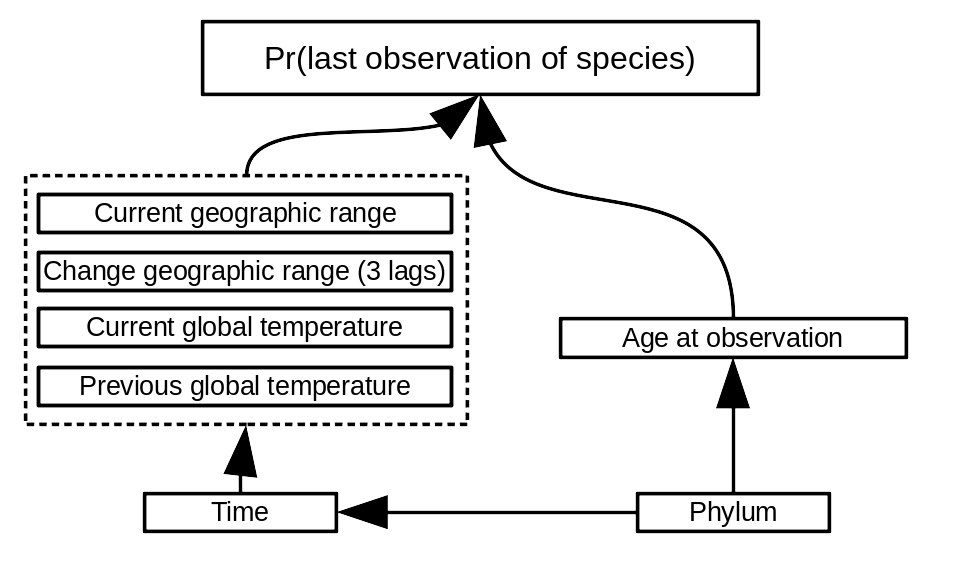
\includegraphics[width=\textwidth,height=\textheight,keepaspectratio=true]{figure/conceptual_diagram}
  \end{center}

\end{frame}


\begin{frame}
  \frametitle{Measuring performance: confusion matrix}

  \begin{center}
    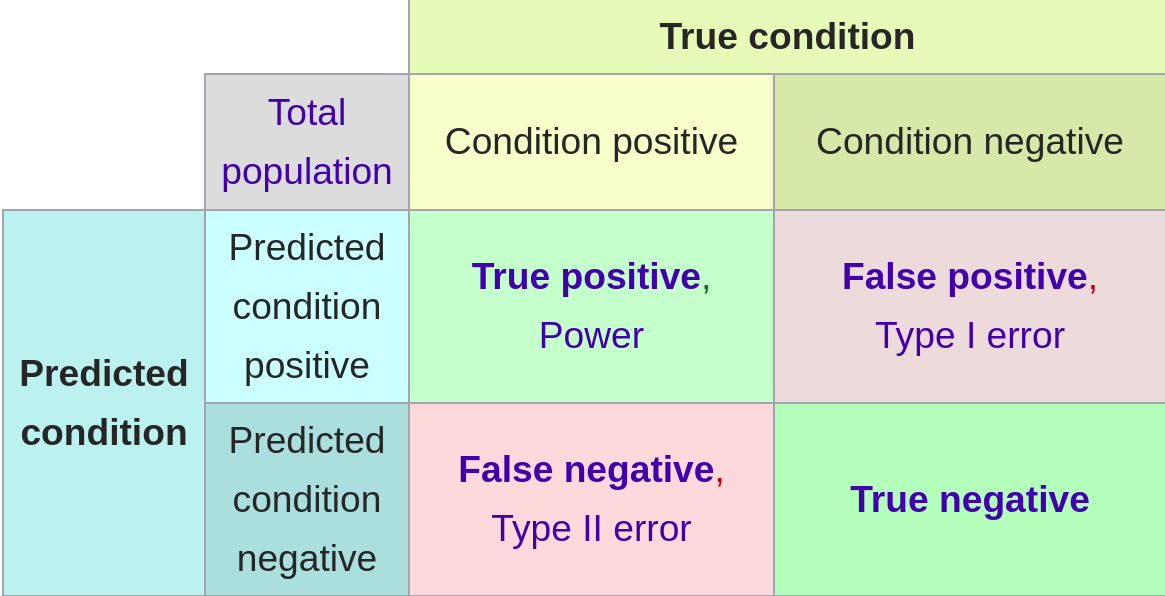
\includegraphics[width=\textwidth,height=0.75\textheight,keepaspectratio=true]{figure/confusion_matrix_wiki}
  \end{center}

  \attrib{\footnotesize{wikimedia}}

\end{frame}
%
%
%\begin{frame}
%  \frametitle{Measuring performance: Receiver Operating Characteristic}
%
%  \begin{center}
%    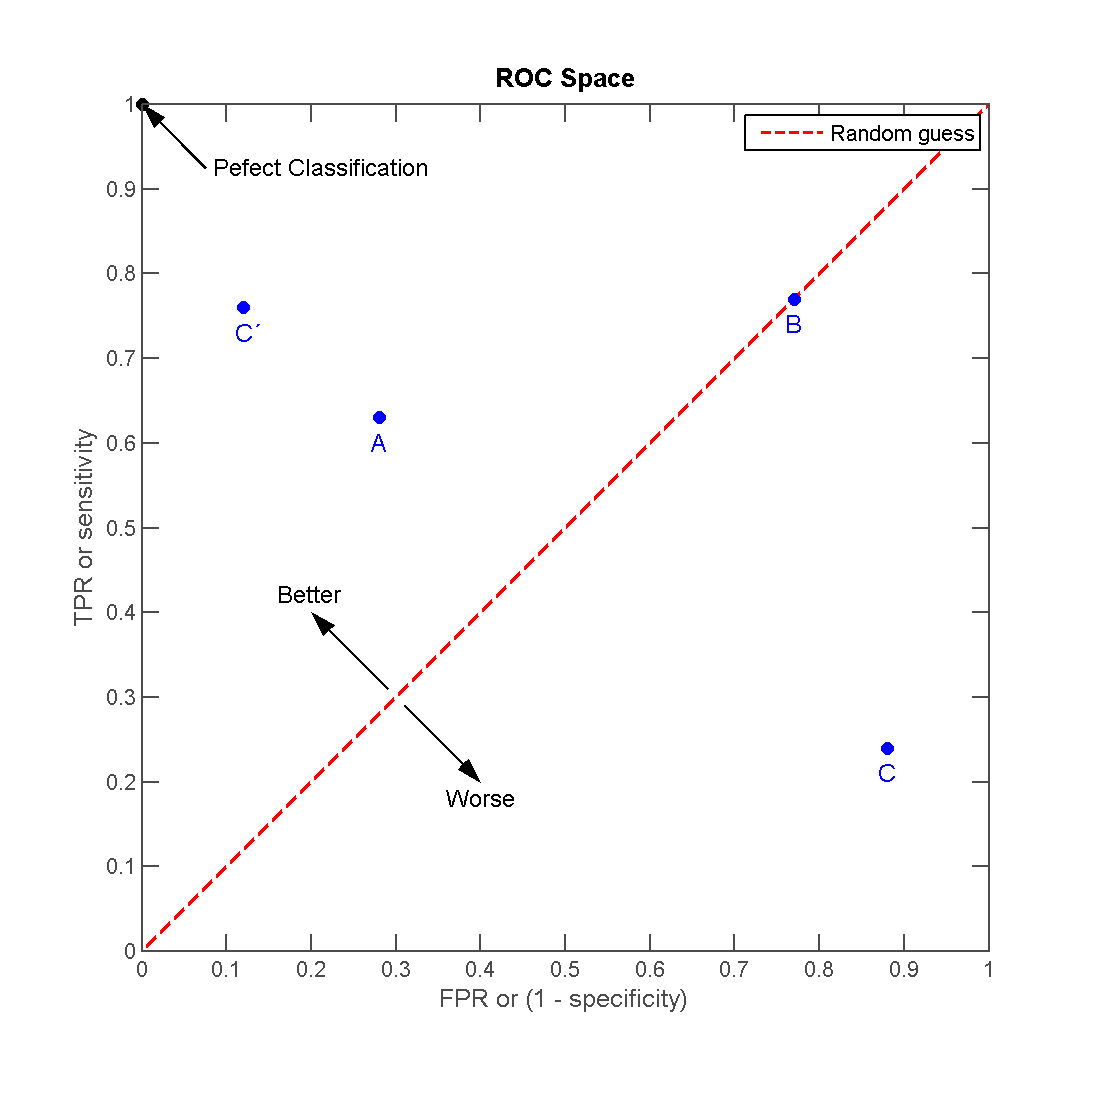
\includegraphics[width=\textwidth,height=0.8\textheight,keepaspectratio=true]{figure/wiki_ROC_space-2}
%  \end{center}
%  
%  \attrib{\footnotesize{wikimedia}}
%
%\end{frame}


\begin{frame}
  \frametitle{Measuring performance: Receiver Operating Characteristic}

  \begin{center}
    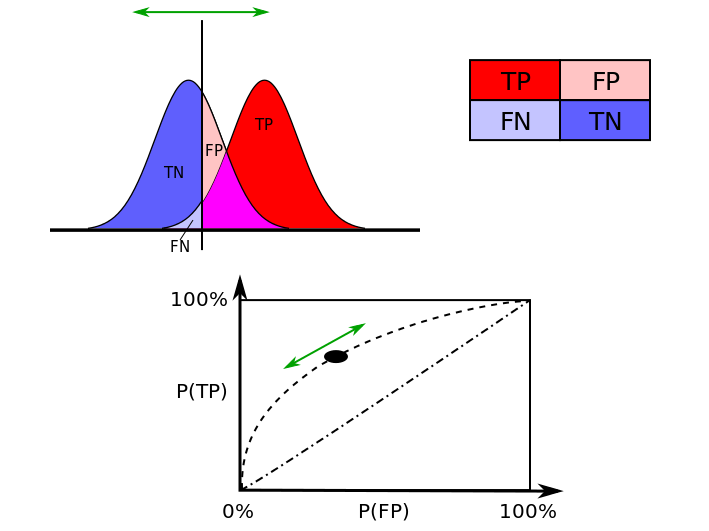
\includegraphics[width=\textwidth,height=0.75\textheight,keepaspectratio=true]{figure/wiki_709px-ROC_curves}
  \end{center}

  \attrib{\footnotesize{wikimedia}}

\end{frame}

\begin{frame}
  \frametitle{Measuring performance: AUC ROC}

  \begin{columns}
    \begin{column}{0.4\textwidth}
      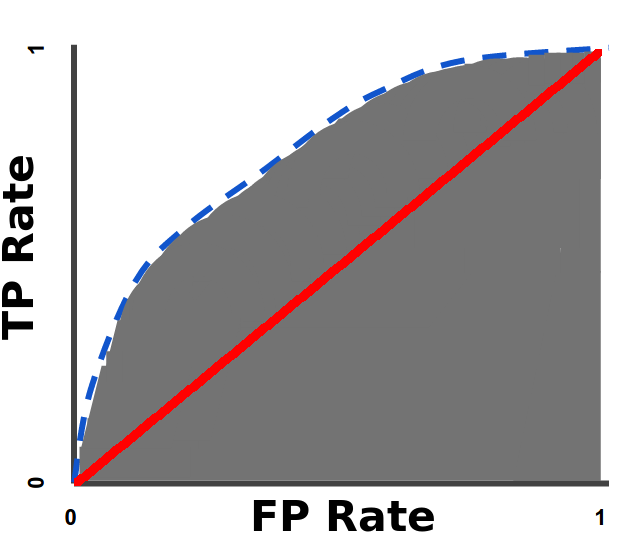
\includegraphics[width=\textwidth,height=\textheight,keepaspectratio=true]{figure/AUC}

      \attrib{\footnotesize{https://goo.gl/91nEpM}}

    \end{column}
    \begin{column}{0.6\textwidth}
      The area represents the probability of correct ranking of a random ``extant''-``extinct'' pair.
      
      \[
        \text{AUC} = 
        \begin{cases} 
          0.5 & \text{non discrimination}\\
          0.6-0.7 & \text{poor} \\
          0.7-0.8 & \text{acceptable/fair} \\
          0.8-0.9 & \text{excellent/good} \\
          > 0.9 & \text{outstanding} \\
        \end{cases}
      \]

    \end{column}
  \end{columns}

\end{frame}

\begin{frame}
  \frametitle{Measuring performance: \textit{k}-fold cross-validation}

  \begin{center}
    \includegraphics[width=\textwidth,height=0.8\textheight,keepaspectratio=true]{figure/ts_cv}
  \end{center}


  \attrib{\footnotesize{Ken Williams, https://goo.gl/qLcfL8}}
\end{frame}

%\begin{frame}
%  \frametitle{In-sample predictive performance, full dataset}
%
%  \begin{center}
%    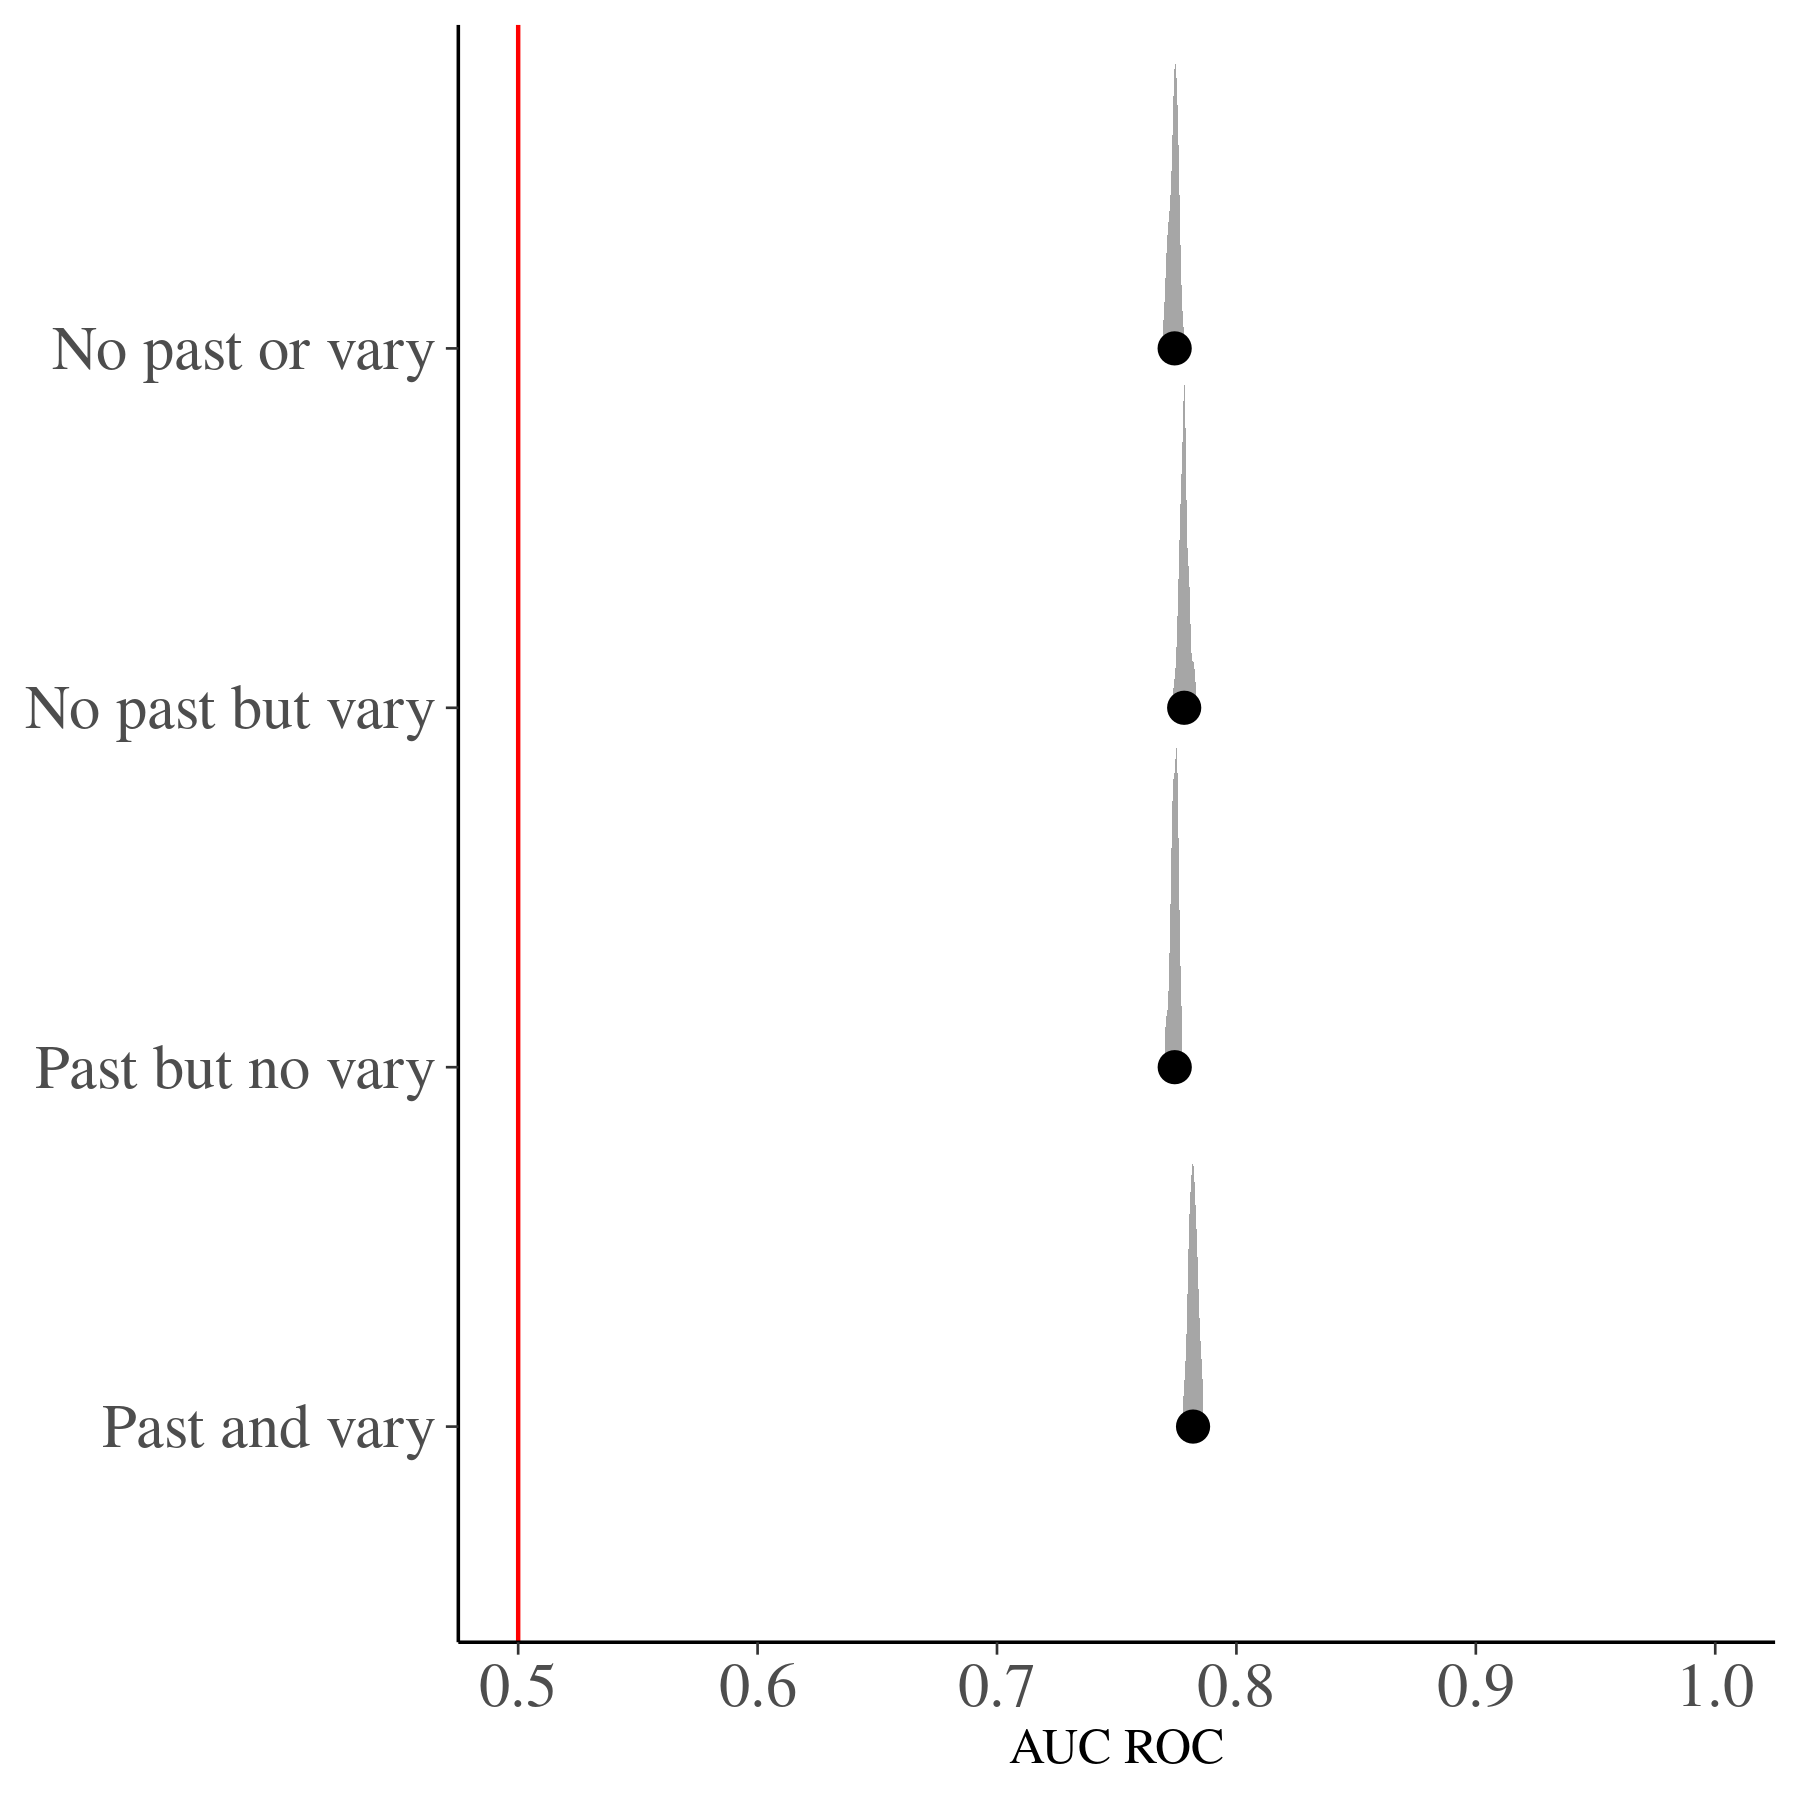
\includegraphics[width=\textwidth,height=0.8\textheight,keepaspectratio=true]{../results/figure/auc_hist_zoom}
%
%    \footnotesize{AUC = 0.7-0.8 acceptable/fair}
%  \end{center}
%
%\end{frame}

% demonstrate as ROC curve?
\begin{frame}
  \frametitle{In-sample predictive performance, full dataset}

  \begin{center}
    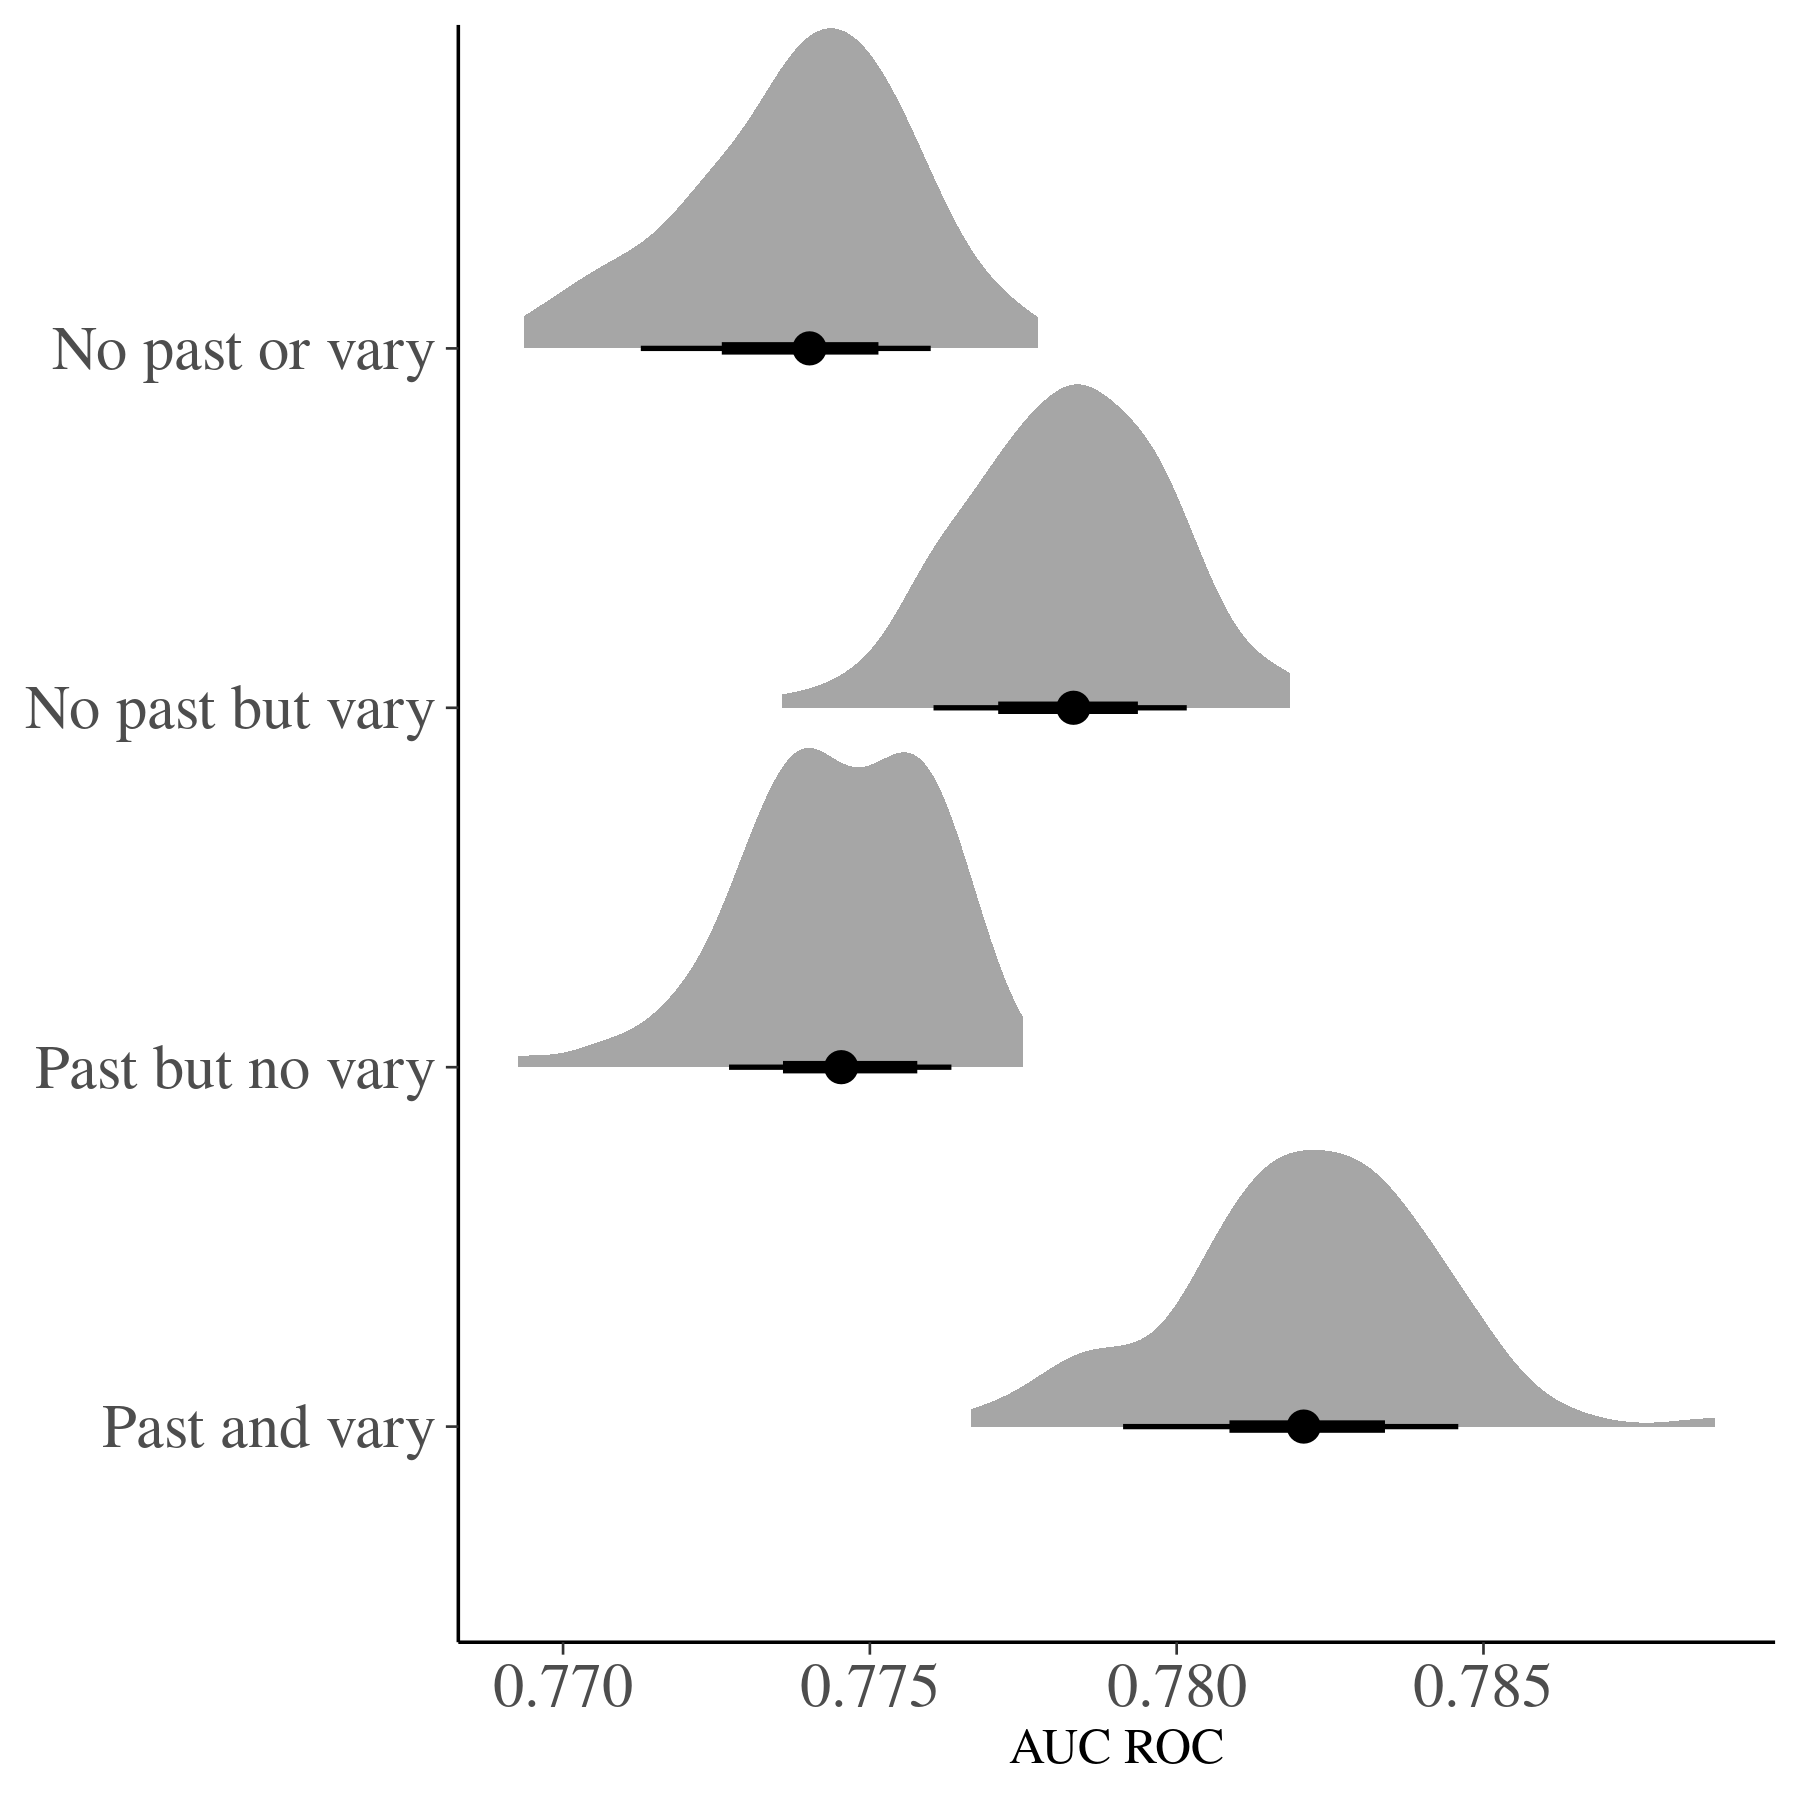
\includegraphics[width=\textwidth,height=0.8\textheight,keepaspectratio=true]{../results/figure/auc_hist_full}

    \footnotesize{AUC = 0.7-0.8 acceptable/fair}
  \end{center}

\end{frame}


\begin{frame}
  \frametitle{In-sample predictive performance, by time and taxa}

  \begin{center}
    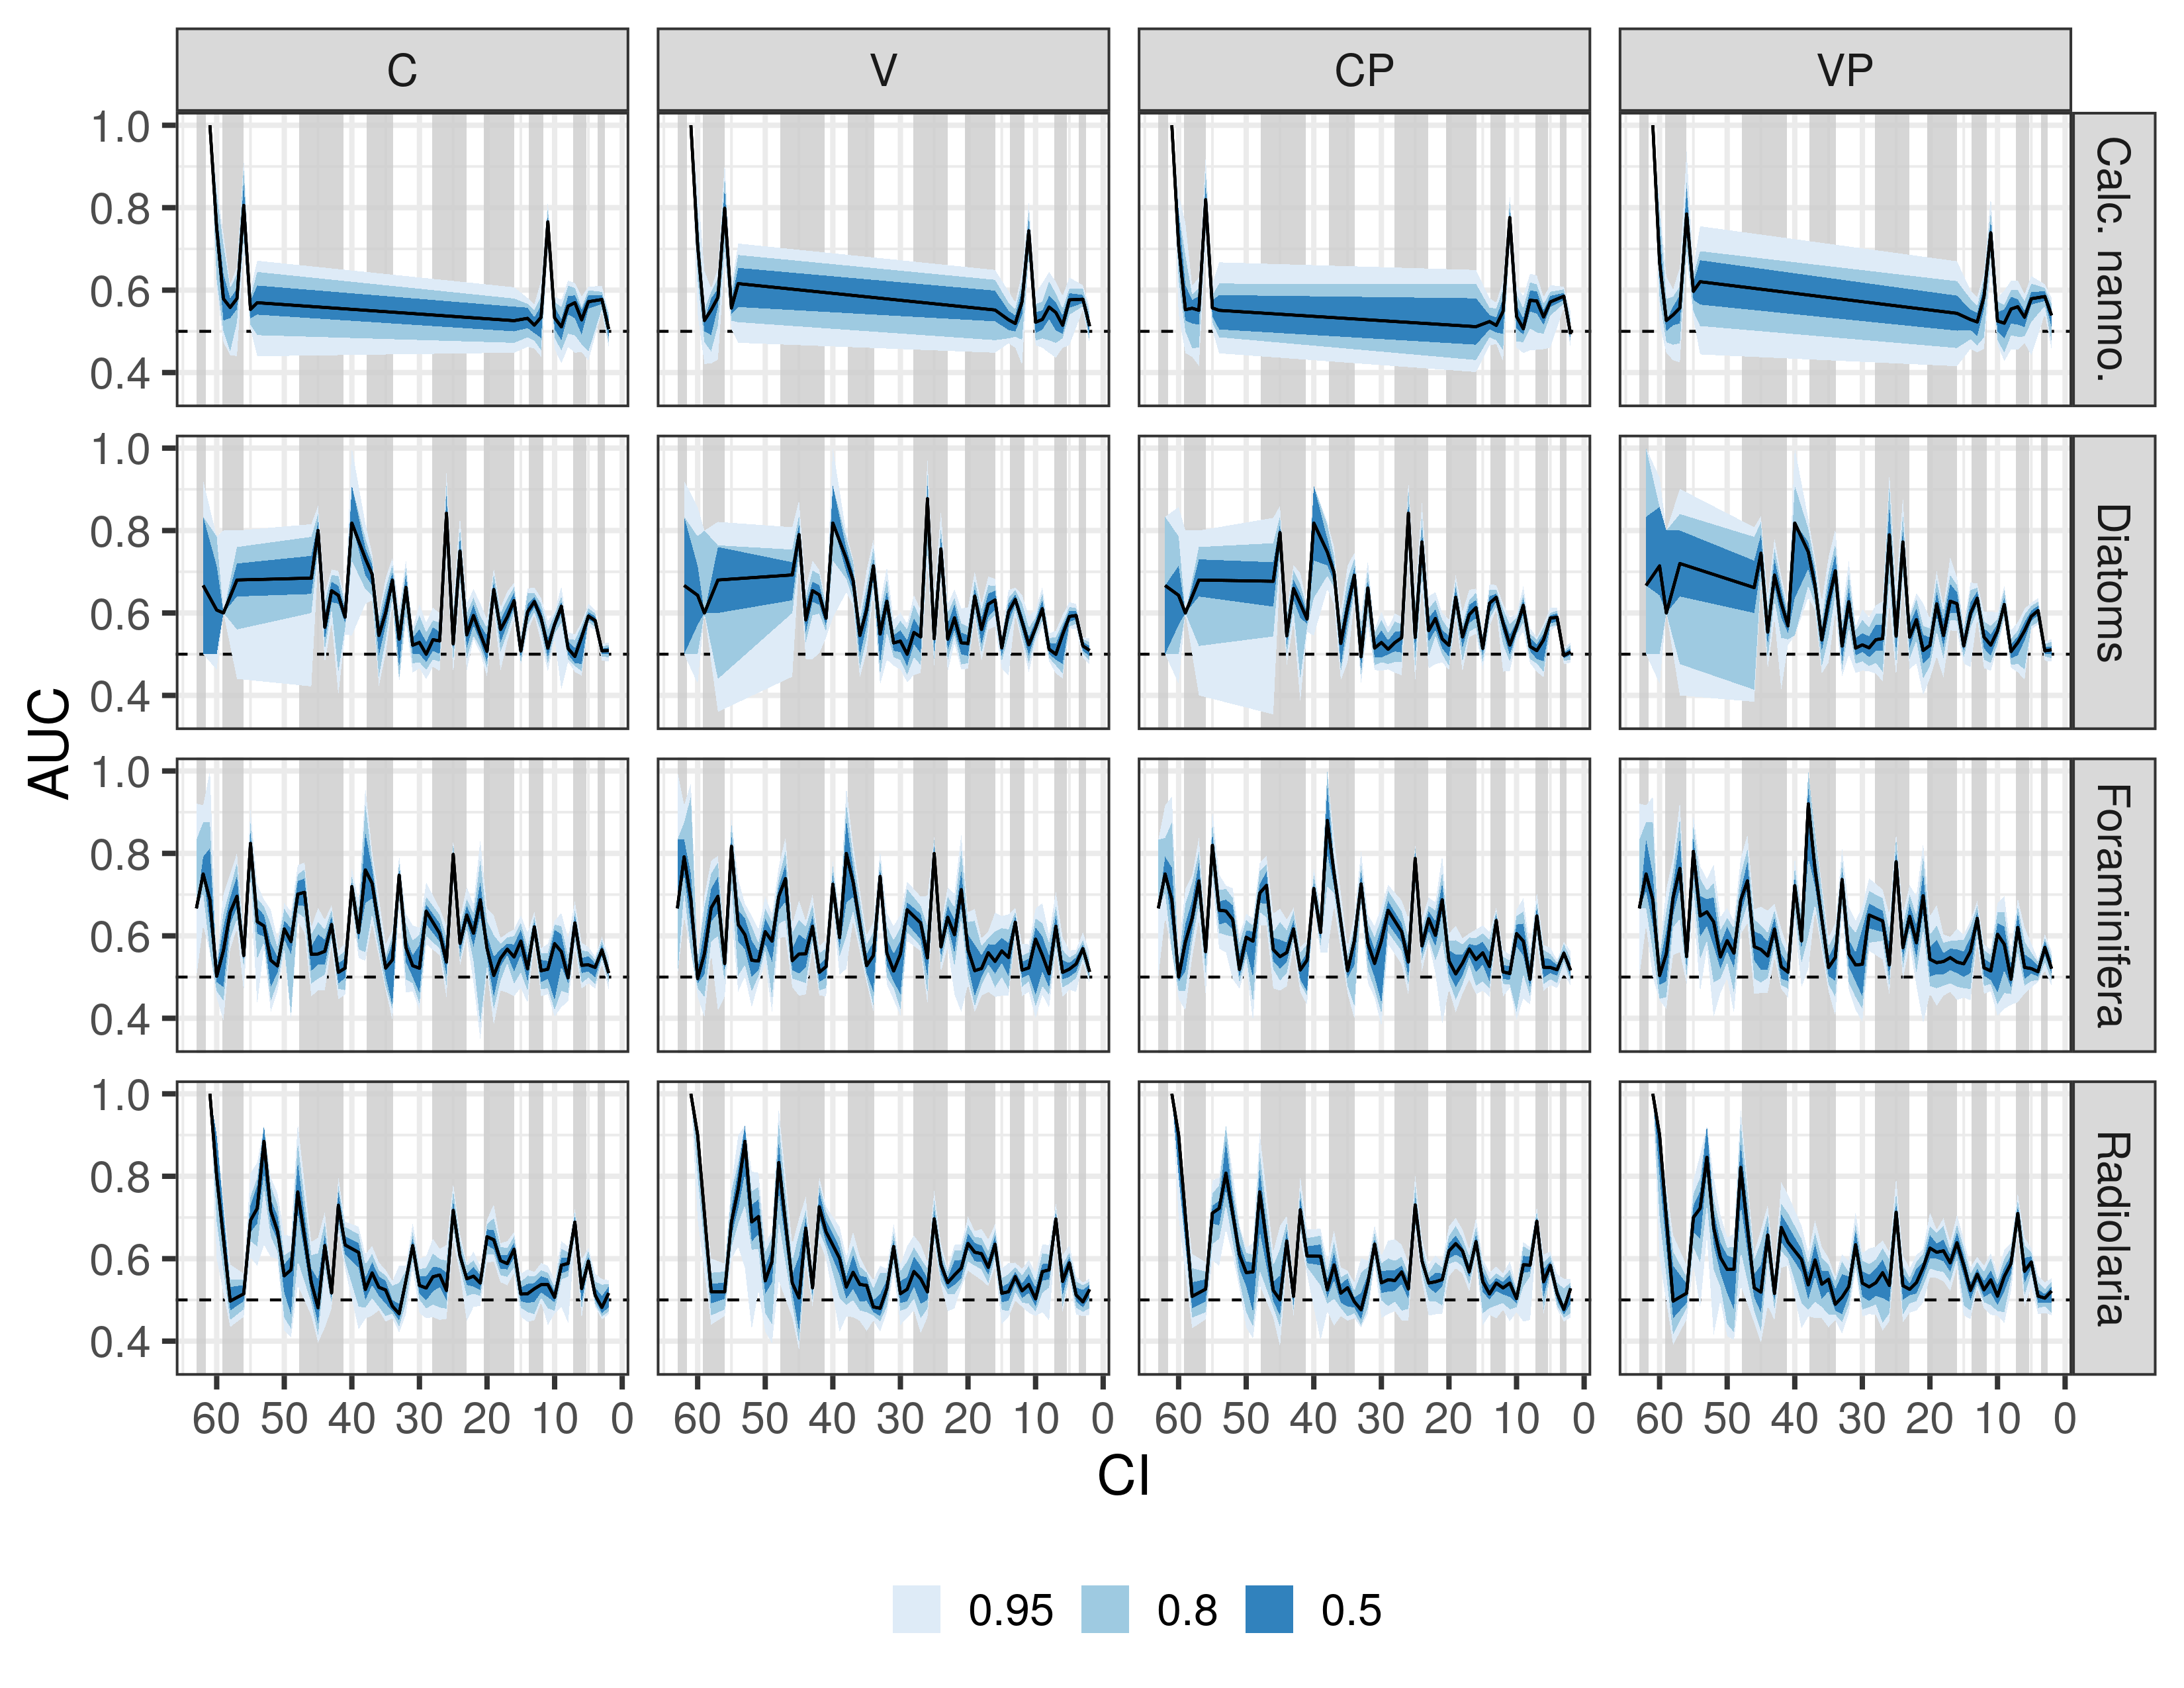
\includegraphics[width=\textwidth,height=0.8\textheight,keepaspectratio=true]{../results/figure/auc_taxon_time_full}
  \end{center}

\end{frame}

\begin{frame}
  \frametitle{Cross-validation results, full dataset}

  \begin{center}
    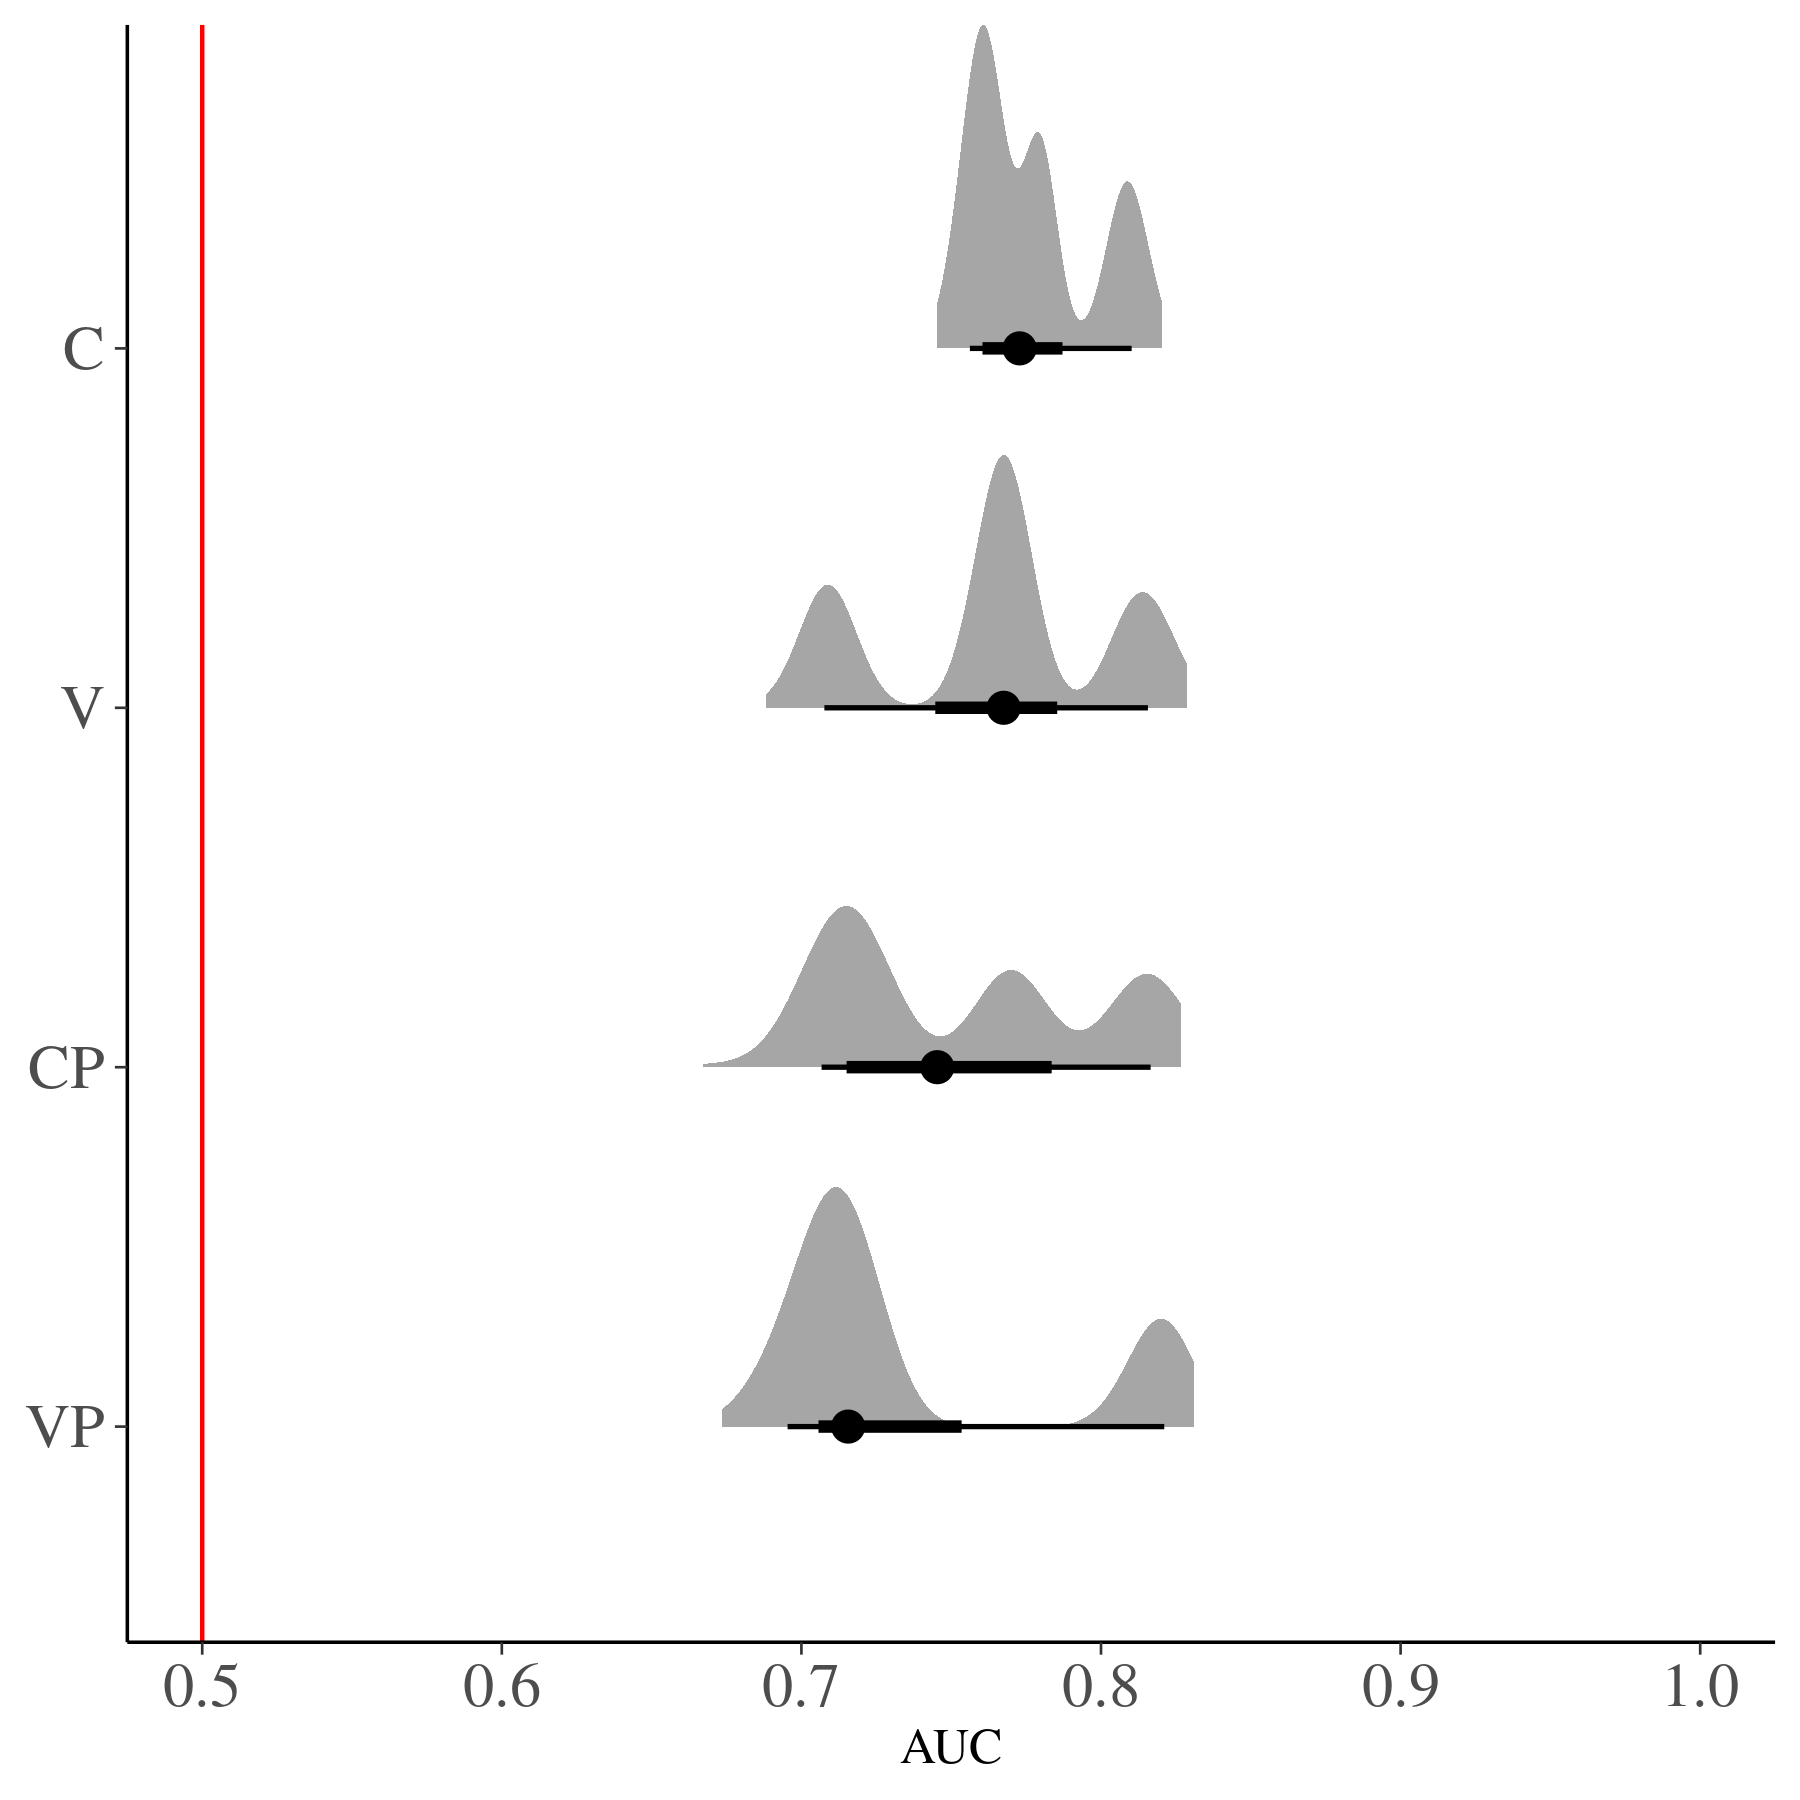
\includegraphics[width=\textwidth,height=0.8\textheight,keepaspectratio=true]{../results/figure/fold_auc_zoom_full}

    \footnotesize{AUC = 0.7-0.8 acceptable/fair}
  \end{center}

\end{frame}

\begin{frame}
  \frametitle{Cross-validation results, by time and taxa}

  \begin{center}
    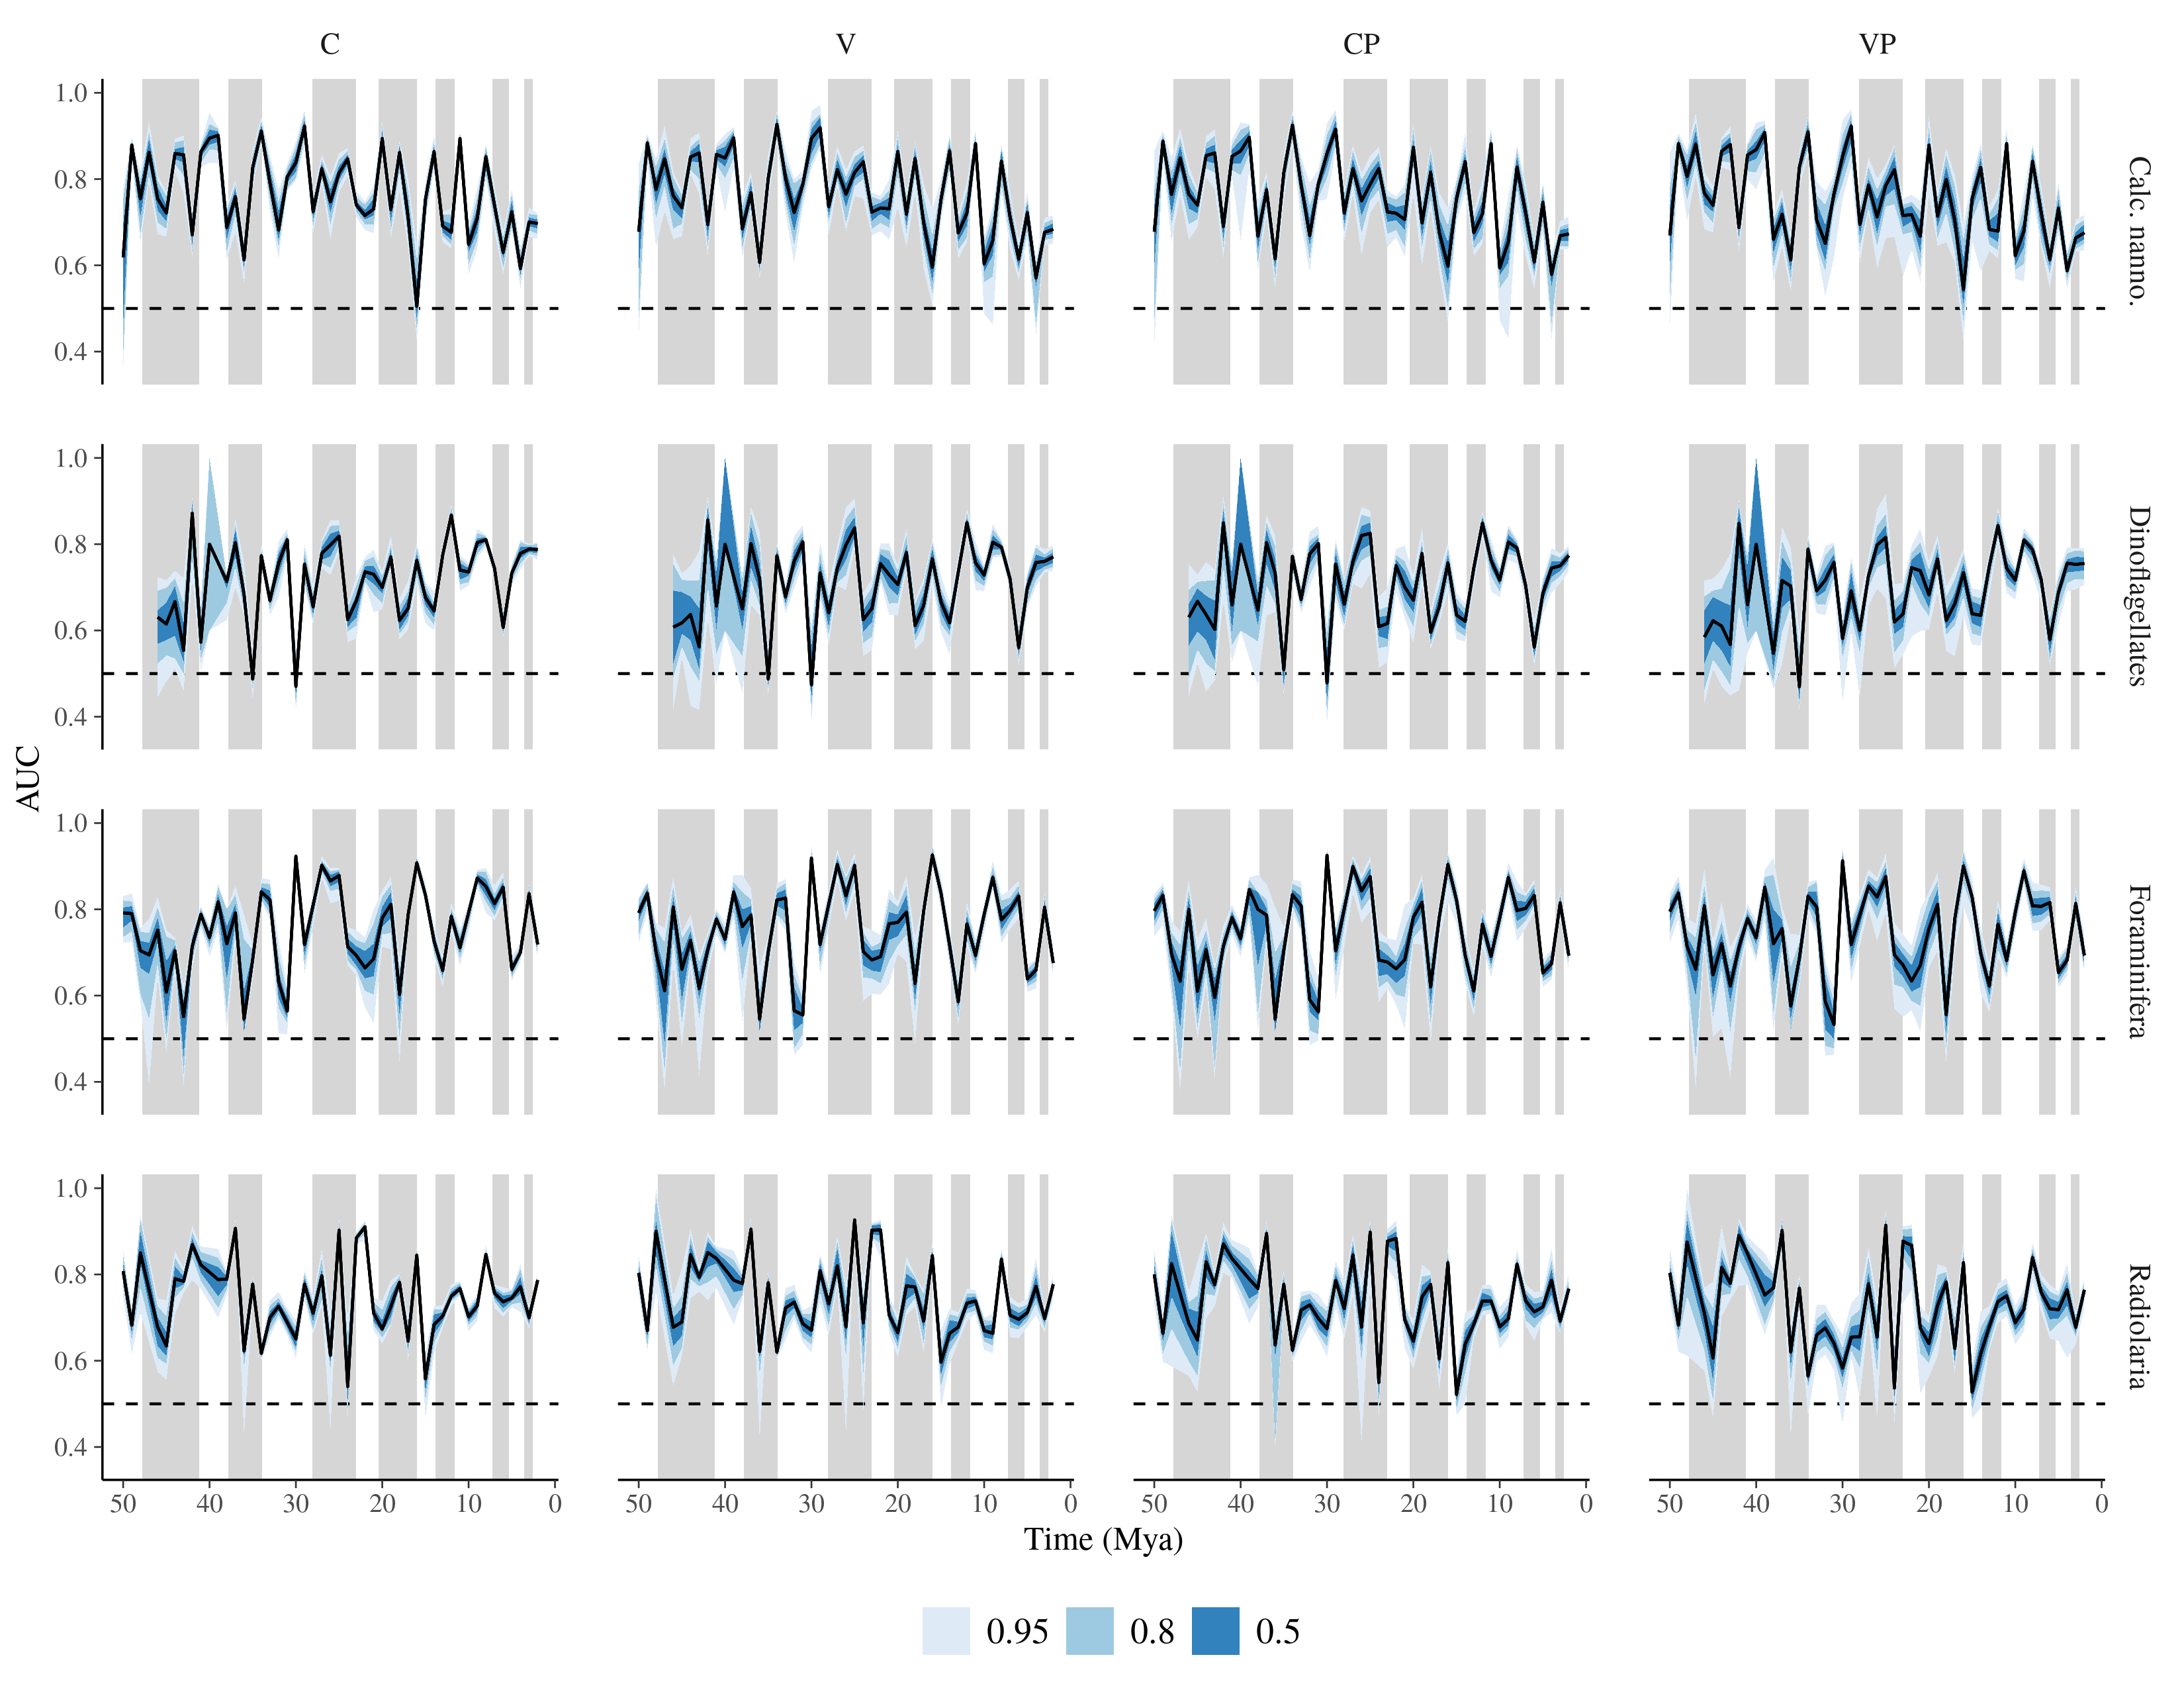
\includegraphics[width=\textwidth,height=0.8\textheight,keepaspectratio=true]{../results/figure/fold_auc_taxon_time_full}
  \end{center}

\end{frame}


\begin{frame}
  \frametitle{Summary}

  \begin{itemize}
    \item \alert{The past matters\dots} 
      \begin{itemize}
        \item Our best supported model includes either our historical covariates or allows all effects to vary over time.
      \end{itemize}
    \item \alert{But not that much\dots}
      \begin{itemize}
        \item Models only average/fair expected out-of-sample performance.
      \end{itemize}
    \item Allowing effects to vary over time is probably preferable to historical covariates -- measures and accounts for variation which is important when predicting extinction in novel environments.
    \item Mechanisms behind changes to geographic range operate at sub-million year scales. Perhaps their effects are weak/masked at million (or greater) year scales.
  \end{itemize}

\end{frame}
  

\begin{frame}

  \begin{center}
    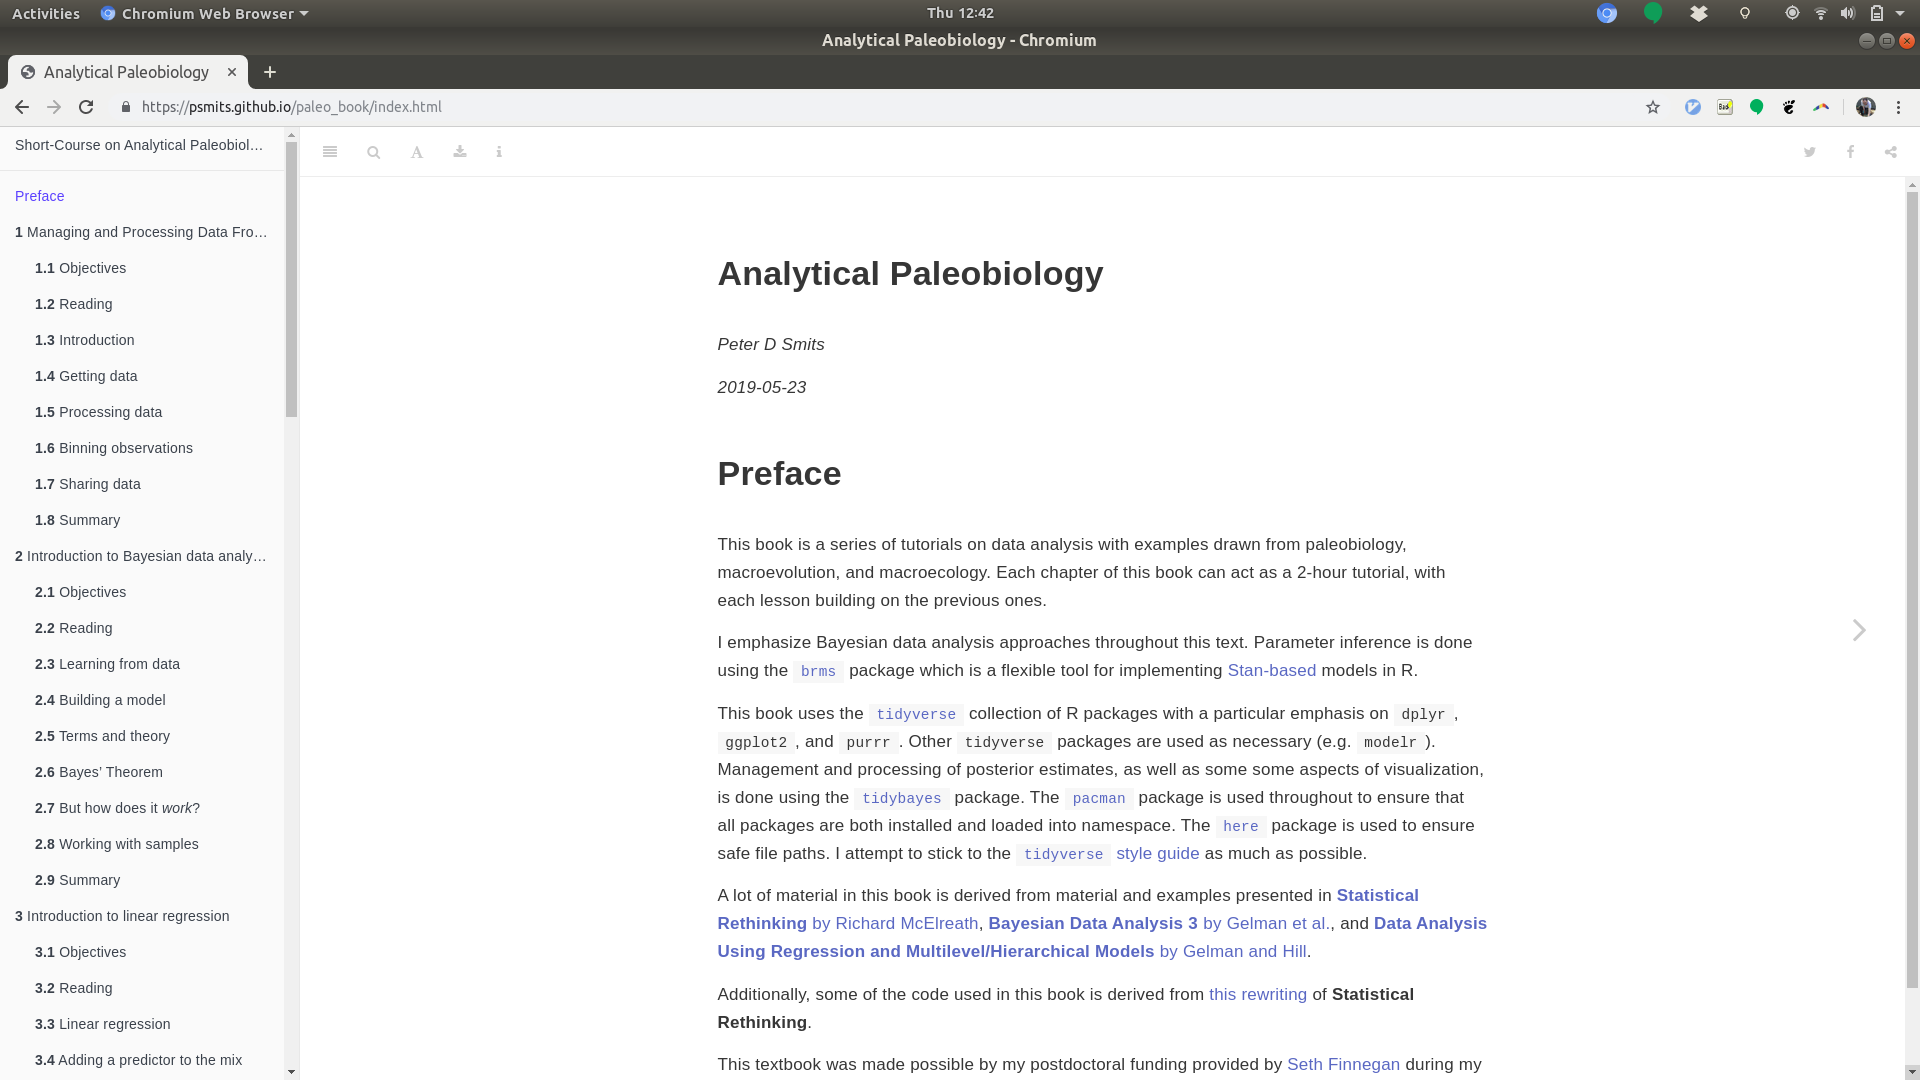
\includegraphics[width=\textwidth,height=0.8\textheight,keepaspectratio=true]{figure/book}

    \Large{https://psmits.github.io/paleo\_book/index.html}
  \end{center}

\end{frame}

\begin{frame}
  \frametitle{Acknowledgements}
  \begin{columns}
    \begin{column}{0.5\textwidth}
      \begin{itemize}
        \item UC Berkeley
          \begin{itemize}
            \item Adiel Klompmaker 
            \item Emily Orzechowski
            \item Larry Taylor
            \item Sara Kahanamoku
            \item Josh Zimmt
          \end{itemize}
        \item University of Oslo
          \begin{itemize}
            \item Franziska Franeck
          \end{itemize}
        \item Neptune DB/MFN - Berlin
          \begin{itemize}
            \item David Lazarus
          \end{itemize}
      \end{itemize}
    \end{column}
    \begin{column}{0.5\textwidth}
      \begin{center}
        
\includegraphics[height=0.15\textheight,width=\textwidth,keepaspectratio=true]{figure/github-logo}

        psmits.github.io/ \hspace*{0.05\textwidth} \textbf{trident}
      \end{center}
      \vspace*{0.02\textheight}
      \begin{center}
        
\includegraphics[height=0.1\textheight,width=0.5\textwidth,keepaspectratio=true]{figure/twitter} 

        @PeterDSmits
      \end{center}

      \vspace*{0.02\textheight}

      \begin{center}
        
\includegraphics[height=0.25\textheight,width=\textwidth,keepaspectratio=true]{figure/nsb_logo}
      \end{center}
    \end{column}
  \end{columns}
\end{frame}

\end{document}

